\documentclass[14pt]{extbook}
\usepackage{multicol, enumerate, enumitem, hyperref, color, soul, setspace, parskip, fancyhdr} %General Packages
\usepackage{amssymb, amsthm, amsmath, bbm, latexsym, units, mathtools} %Math Packages
\everymath{\displaystyle} %All math in Display Style
% Packages with additional options
\usepackage[headsep=0.5cm,headheight=12pt, left=1 in,right= 1 in,top= 1 in,bottom= 1 in]{geometry}
\usepackage[usenames,dvipsnames]{xcolor}
\usepackage{dashrule}  % Package to use the command below to create lines between items
\newcommand{\litem}[1]{\item#1\hspace*{-1cm}\rule{\textwidth}{0.4pt}}
\pagestyle{fancy}
\lhead{Makeup Progress Quiz -1}
\chead{}
\rhead{Version A}
\lfoot{7547-2949}
\cfoot{}
\rfoot{Fall 2020}
\begin{document}

\begin{enumerate}
\litem{
Determine the horizontal and/or oblique asymptotes in the rational function below.\[ f(x) = \frac{8x^{3} +18 x^{2} -15 x -25}{2x^{2} +x -10} \]\begin{enumerate}[label=\Alph*.]
\item \( \text{Horizontal Asymptote at } y = 2.0 \)
\item \( \text{Horizontal Asymptote of } y = 2.0 \text{ and Oblique Asymptote of } y = 4x + 7 \)
\item \( \text{Oblique Asymptote of } y = 4x + 7. \)
\item \( \text{Horizontal Asymptote of } y = 4.0  \)
\item \( \text{Horizontal Asymptote of } y = 4.0 \text{ and Oblique Asymptote of } y = 4x + 7 \)

\end{enumerate} }
\litem{
Determine the horizontal and/or oblique asymptotes in the rational function below.\[ f(x) = \frac{30x^{3} -61 x^{2} -18 x + 40}{20x^{3} +57 x^{2} -62 x -40} \]\begin{enumerate}[label=\Alph*.]
\item \( \text{Vertical Asymptote of } y = 2  \)
\item \( \text{Horizontal Asymptote of } y = 0  \)
\item \( \text{None of the above} \)
\item \( \text{Horizontal Asymptote of } y = 1.500  \)
\item \( \text{Vertical Asymptote of } y = -1.250  \)

\end{enumerate} }
\litem{
Which of the following functions \textit{could} be the graph below?
\begin{center}
    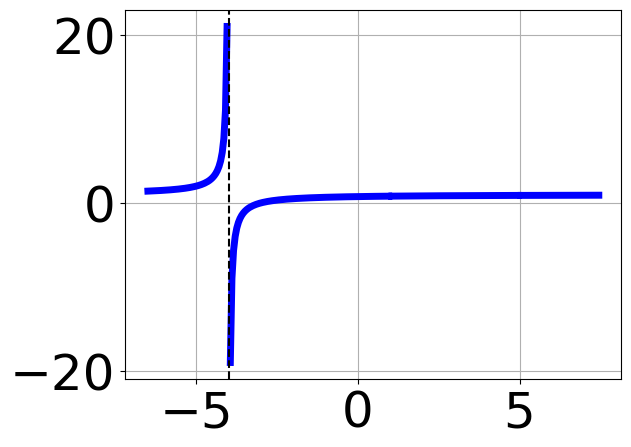
\includegraphics[width=0.5\textwidth]{../Figures/identifyGraphOfRationalFunctionA.png}
\end{center}
\begin{enumerate}[label=\Alph*.]
\item \( f(x)=\frac{x^{3} +8 x^{2} +x -42}{x^{3} -2 x^{2} -19 x + 20} \)
\item \( f(x)=\frac{x^{3} +3 x^{2} -13 x -15}{x^{3} +2 x^{2} -19 x -20} \)
\item \( f(x)=\frac{x^{3} -3 x^{2} -13 x + 15}{x^{3} -2 x^{2} -19 x + 20} \)
\item \( f(x)=\frac{x^{3} +3 x^{2} -13 x -15}{x^{3} +2 x^{2} -19 x -20} \)
\item \( \text{None of the above are possible equations for the graph.} \)

\end{enumerate} }
\litem{
Determine the horizontal and/or oblique asymptotes in the rational function below.\[ f(x) = \frac{8x^{3} +46 x^{2} +41 x -60}{4x^{2} +17 x -15} \]\begin{enumerate}[label=\Alph*.]
\item \( \text{Oblique Asymptote of } y = 2x + 3. \)
\item \( \text{Horizontal Asymptote of } y = -5.0 \text{ and Oblique Asymptote of } y = 2x + 3 \)
\item \( \text{Horizontal Asymptote of } y = 2.0 \text{ and Oblique Asymptote of } y = 2x + 3 \)
\item \( \text{Horizontal Asymptote of } y = 2.0  \)
\item \( \text{Horizontal Asymptote at } y = -5.0 \)

\end{enumerate} }
\litem{
Determine the vertical asymptotes and holes in the rational function below.\[ f(x) = \frac{9x^{3} +48 x^{2} +73 x + 30}{6x^{2} -5 x -25} \]\begin{enumerate}[label=\Alph*.]
\item \( \text{Holes at } x = 2.5 \text{ and } x = -1.667 \text{ with no vertical asymptotes.} \)
\item \( \text{Vertical Asymptote of } x = 2.5 \text{ and hole at } x = -1.667 \)
\item \( \text{Vertical Asymptotes of } x = 2.5 \text{ and } x = -0.667 \text{ with a hole at } x = -1.667 \)
\item \( \text{Vertical Asymptote of } x = 1.5 \text{ and hole at } x = -1.667 \)
\item \( \text{Vertical Asymptotes of } x = 2.5 \text{ and } x = -1.667 \text{ with no holes.} \)

\end{enumerate} }
\litem{
Determine the vertical asymptotes and holes in the rational function below.\[ f(x) = \frac{9x^{3} -30 x^{2} +31 x -10}{6x^{2} +11 x -10} \]\begin{enumerate}[label=\Alph*.]
\item \( \text{Vertical Asymptote of } x = -2.5 \text{ and hole at } x = 0.667 \)
\item \( \text{Vertical Asymptotes of } x = -2.5 \text{ and } x = 1.667 \text{ with a hole at } x = 0.667 \)
\item \( \text{Vertical Asymptote of } x = 1.5 \text{ and hole at } x = 0.667 \)
\item \( \text{Holes at } x = -2.5 \text{ and } x = 0.667 \text{ with no vertical asymptotes.} \)
\item \( \text{Vertical Asymptotes of } x = -2.5 \text{ and } x = 0.667 \text{ with no holes.} \)

\end{enumerate} }
\litem{
Determine the horizontal and/or oblique asymptotes in the rational function below.\[ f(x) = \frac{3x^{2} -11 x -20}{12x^{3} -17 x^{2} -104 x -80} \]\begin{enumerate}[label=\Alph*.]
\item \( \text{Horizontal Asymptote of } y = 0.250 \text{ and Oblique Asymptote of } y = 4x + 9 \)
\item \( \text{Horizontal Asymptote at } y = 5.000 \)
\item \( \text{Horizontal Asymptote of } y = 0 \)
\item \( \text{Horizontal Asymptote of } y = 0.250  \)
\item \( \text{Oblique Asymptote of } y = 4x + 9. \)

\end{enumerate} }
\litem{
Which of the following functions \textit{could} be the graph below?
\begin{center}
    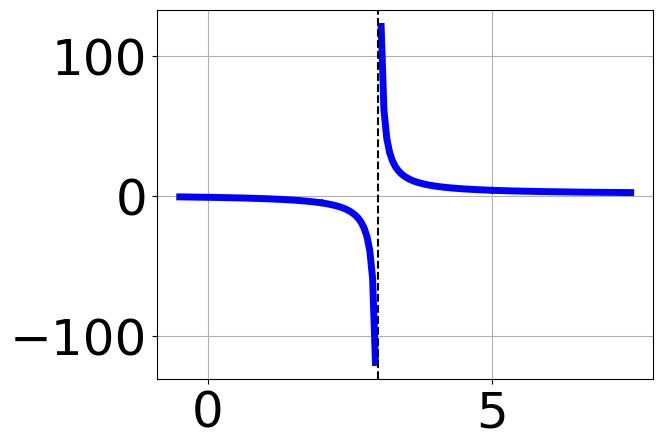
\includegraphics[width=0.5\textwidth]{../Figures/identifyGraphOfRationalFunctionCopyA.png}
\end{center}
\begin{enumerate}[label=\Alph*.]
\item \( f(x)=\frac{x^{3} +4 x^{2} -11 x -30}{x^{3} +10 x^{2} +31 x + 30} \)
\item \( f(x)=\frac{x^{3} -4 x^{2} -11 x + 30}{x^{3} -10 x^{2} +31 x -30} \)
\item \( f(x)=\frac{x^{3} +13 x^{2} +54 x + 72}{x^{3} -10 x^{2} +31 x -30} \)
\item \( f(x)=\frac{x^{3} +4 x^{2} -11 x -30}{x^{3} +10 x^{2} +31 x + 30} \)
\item \( \text{None of the above are possible equations for the graph.} \)

\end{enumerate} }
\litem{
Determine the vertical asymptotes and holes in the rational function below.\[ f(x) = \frac{16x^{3} +64 x^{2} +79 x + 30}{16x^{2} -9} \]\begin{enumerate}[label=\Alph*.]
\item \( \text{Vertical Asymptotes of } x = 0.75 \text{ and } x = -1.25 \text{ with a hole at } x = -0.75 \)
\item \( \text{Vertical Asymptote of } x = 0.75 \text{ and hole at } x = -0.75 \)
\item \( \text{Vertical Asymptotes of } x = 0.75 \text{ and } x = -0.75 \text{ with no holes.} \)
\item \( \text{Vertical Asymptote of } x = 1.0 \text{ and hole at } x = -0.75 \)
\item \( \text{Holes at } x = 0.75 \text{ and } x = -0.75 \text{ with no vertical asymptotes.} \)

\end{enumerate} }
\litem{
Determine the vertical asymptotes and holes in the rational function below.\[ f(x) = \frac{6x^{3} -25 x^{2} -11 x + 60}{9x^{2} -25} \]\begin{enumerate}[label=\Alph*.]
\item \( \text{Vertical Asymptotes of } x = -1.667 \text{ and } x = 1.667 \text{ with no holes.} \)
\item \( \text{Vertical Asymptote of } x = 0.667 \text{ and hole at } x = 1.667 \)
\item \( \text{Vertical Asymptote of } x = -1.667 \text{ and hole at } x = 1.667 \)
\item \( \text{Holes at } x = -1.667 \text{ and } x = 1.667 \text{ with no vertical asymptotes.} \)
\item \( \text{Vertical Asymptotes of } x = -1.667 \text{ and } x = -1.5 \text{ with a hole at } x = 1.667 \)

\end{enumerate} }
\end{enumerate}

\end{document}